\section{La sustentation et l'aile}

\subsection{L'aile : description}

\subsubsection{Description générale}
Toute aile est composée de plusieurs parties distinctes :
\begin{itemize}
	\item L'\gls{intrados} est la partie inférieure de l'aile. Lorsque l'aile se déplace dans une masse d'air, l'intrados est le siège d'une surpression.
	\item L'\gls{extrados} est la partie supérieure de l'aile. Lorsque l'aile se déplace dans une masse d'air, l'extrados est le siège d'une dépression (l'aile est aspirée vers le haut).
	\item Le \gls{bord d'attaque} \anglais{leading edge} est le point le plus en avant d'un profil d'aile. C'est à ce point que l'air entrera en contact en premier avec l'aile. Il s'agit généralement d'une surface  courbe.
	\item Le \gls{bord de fuite} \anglais{trailing edge} est le point le plus en arrière d'un profil d'aile.  Il s'agit généralement d'une surface pointue.
\end{itemize}

	\begin{figure}[H]
  	\centering
    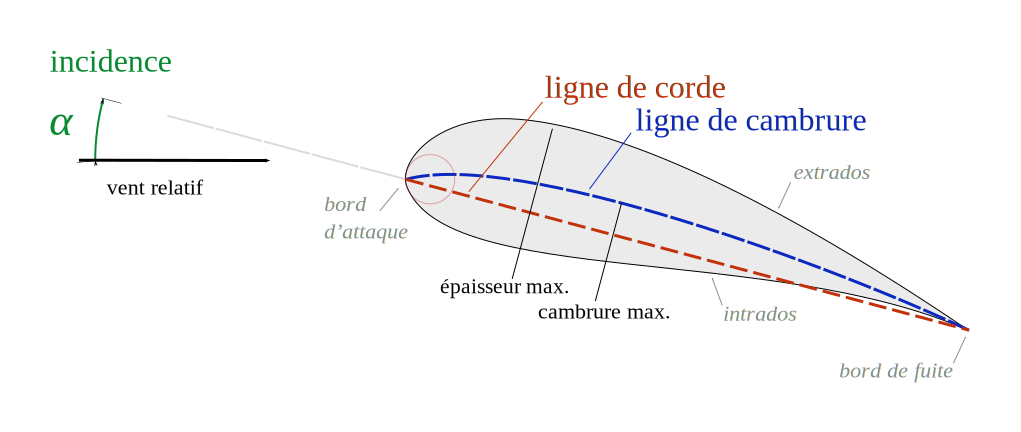
\includegraphics[width=0.8\textwidth]{04-Aerodynamique/img/profilAile}
  	\legende{Profil d'une aile}{img:profilAile}
	\end{figure}	
	
	\astuce{Pour se souvenir ou sont situés l'intrados et l'extrados : que l'avion vol à plat, l'extrados fait face à l'extérieur de la planète, l'intrados regarde vers l'intérieur de la planète.} 	

